% Chapter 06 - Postop CRP and complications

\chapter{An investigation into the relationship between postoperative systemic inflammation and complications after pancreaticoduodenectomy.}
\label{ch_survival}

\lhead{Chapter \ref{ch_survival}. \emph{Postoperative CRP and complications}} % This is for the header on each page - perhaps a shortened title

\clearpage
%----------------------------------------------------------------------------------------
\section{Introduction}
Pancreaticoduodenectomy is associated with significant morbidity in spite of advances in patient selection, perioperative care and surgical technique. Early identification of complications can help improve outcomes by better allocation of critical care resources as well as goal-directed therapy. Postoperative pancreatic fistula is one of the most dreaded complications after a pancreaticoduodenectomy and can lead to a cascade of other complications including delayed haemorrhage, infected intra-abdominal collections, delayed gastric emptying, prolonged hospitalisation and in some cases, death. The International Study Group for Pancreatic Fistula (ISGPF) have not only defined what constitutes a post-operative pancreatic fistula but have also graded the severity of this complication based on its impact on the management of the patient. However, these definitions are applied after the event and there is no clear way of predicting the severity of complications.

Postoperative CRP levels have been shown to predict infectious complications after colorectal surgery as well as oesophago-gastric surgery. It has been postulated that an unmitigated and exaggerated systemic inflammatory response in the early postoperative period is followed by a compensatory anti-inflammatory response that predisposes the patient to sepsis and impaired healing. The role of postoperative CRP in predicting the severity of complications after major pancreatic surgery has not been reported before. Stratifying patients based on the predicted severity of complications will allow identifying low risk patients who will be suitable to continue on enhanced recovery pathways and high risk patients who may require prolonged critical care, prolonged hospitalisation or further interventions.

The aim of this study was to investigate the association between postoperative systemic inflammation and severity of complications after pancreaticoduodenectomy.

\section{Methods}
\todo{Check dates for this study}
Patients who underwent elective pancreaticoduodenectomy between January 2008 and July 2012 were included in the study. Patients who underwent only a trial dissection or trial dissection and surgical bypass during this period were excluded. All patients were given antibiotic prophylaxis at induction and this was continued for 24 hours after surgery. All patients had general anaesthesia supplemented either with patient-controlled epidural analgesia or spinal diamorphine and patient-controlled opiate analgesia for postoperative pain relief. Patients were routinely admitted to the surgical high dependency unit where a standardised regimen was followed for early mobilisation, chest physiotherapy and early enteral nutrition. All patients had one or two surgical drain(s) placed at the time of surgery which were removed at the clinician's discretion during the postoperative period based on the presence or absence of postoperative pancreatic fistula or other intra-abdominal collections. 

Patients had routine measurements of inflammatory markers including C-reactive protein (CRP) and differential white cell counts from the day before surgery and every day for at least a week after surgery. These results including the preoperative blood tests and the postoperative blood tests for the first 7 days after surgery were collected from the hospital laboratory databases.

All complications were discussed at a weekly morbidity meeting and prospectively recorded in an electronic database.  The diagnosis and grading of pancreas-specific complications including postoperative pancreatic fistula (POPF, Section \ref{sec:ch_intro_POPF}) and post-pancreatectomy haemorrhage (PPH, Section \ref{sec:ch_intro_PPH}) were made according to the International Study Group classifications as shown in Table \ref{table:isgps_popf} and Table \ref{table:isgps_pph} on p\pageref{table:isgps_popf} respectively.

All other complications were graded using the Clavien-Dindo system as shown in Table \ref{table:clavien-dindo}. This allows the grading of the severity of the complications based on the magnitude of the intervention(s) required to treat them. Postoperative mortality was defined as death within 30-days of the operation or while still in hospital after the operation. Re-intervention in the form of radiological, endoscopic or surgical procedures was recorded prospectively.

\subsection{Statistics}
Mann-Whitney U test was used to compare the distribution of postoperative CRP (as a continuous variable) in patients who had a complication and those who did not. Data are presented as median (inter-quartile range, IQR) unless otherwise specified. Line plots with error bars depicting 95\% confidence intervals are used to depict the trends in CRP over time across different patient groups. 

Receiver operating characteristic (ROC) analysis was used to identify the optimum thresholds for postoperative CRP for predicting infectious complications with a preference for thresholds that had a greater negative predictive value. Patients were categorised using these thresholds to analyse the relationship between CRP (as a categorical variable) and re-operation, hospital stay, critical care stay, number of critical care admissions as well as postoperative mortality using the Chi-square test of proportions. 

SPSS software (Version 22.0; IBM, USA) was used to perform statistical analysis.
Effects were considered significant at $\alpha \leq0.05$. 

\todo{Complete this section - most of this can be modified from the stats sections in other chapters}


\section{Results}
Pancreaticoduodenectomy was performed in 188 patients (126 male, 67\%) during the study period. The median age was 63.5 years (IQR 54 - 70 years). 79 (42\%) patients were over the age of 65 years. 

Post-operative pancreatic fistula (POPF) as defined by the International Study Group for Pancreatic Fistula (ISGPF) occurred in 61 (33\%) patients. Of these patients, 18 (10.1\%) had a Grade A POPF, 25 (13.3\%) had a Grade B POPF and 18 (9.6\%) had a Grade C POPF. Significant infectious complications of Clavien-Dindo grade 3 or higher occurred in 84 patients. Infectious complications were more common in patients with age $>$65 years (35.6\% vs 50.0\%, p=0.046) and $\dot{V}_{O_2}$AT$<$10 mls/kg/min (28.8\% vs. 52.4\%, p=0.006) were significantly associated with infectious complications. Gender, body mass index, smoking status, modified Glasgow Prognostic Score, preoperative serum bilirubin and POSSUM physiology score were not associated with infectious complications.

Infectious complications were also significantly associated with other complications including post-operative pancreatic fistula, post-pancreatectomy haemorrhage, length of stay in hospital, critical care stay, number of critical care admissions, reoperation rates and in-hospital mortality. (Table \ref{table:crp_comp_infect_vs_other_complications})

%12/07/15 - Started this table
\begin{table}[p]
	\centering
	\caption{The relationship between preoperative clinicopathological characteristics and infective complications in patients undergoing pancreaticoduodenectomy.}
	\label{table:crp_comp_preop_factors}
	\renewcommand{\arraystretch}{1.5} %Increases space between rows
	\setlength{\tabcolsep}{12pt} %sets the space between columns
	\begin{tabular}{|l l c c c|}
		\hline
		                  &          & \multicolumn{2}{c}{Infective complication} &  \\
		                  &          & CD 0 - 2    & CD 3 - 5                       & p     \\ \hline
		Age               & $\leq$65 & 67 (64.4\%) & 42 (50.0\%)                    & 0.046 \\
		                  & $>$65    & 37 (35.6\%) & 42 (50.0\%)                    &  \\
		Gender            & Male     & 70 (67.3\%) & 56 (66.7\% )                   & 0.926 \\
		                  & Female   & 34 (32.7\%) & 28 (33.3\%)                    &  \\
		BMI               & $\leq$25 & 48 (50.5\%) & 37 (46.3\%)                    & 0.573 \\
		                  & $>$25    & 47 (49.5\%) & 43 (53.8\%)                    &  \\
		Smoking           & No       & 53 (62.4\%) & 44 (59.5\%)                    & 0.709 \\
		                  & Yes      & 32 (37.6\%) & 30 (40.5\%)                    &  \\
		mGPS              & 0        & 67 (64.4\%) & 49 (59.8\%)                    & 0.570 \\
		                  & 1        & 7 (6.7\%)   & 9 (11.0\%)                     &  \\
		                  & 2        & 30 (28.8\%) & 24 (29.3\%)                    &  \\
		Bilirubin         & $\leq$35 & 66 (63.5\%) & 47 (56.0\%)                    & 0.574 \\
		                  & 35 - 250 & 22 (21.2\%) & 22 (26.2\%)                    &  \\
		                  & $>$250   & 16 (15.4\%) & 15 (17.9\%)                    &  \\
		$\dot{V}_{O_2}$AT & $\geq$10 & 47 (71.2\%) & 30 (47.6\%)                    & 0.006 \\
		                  & $<$10    & 19(28.8\%)  & 33 (52.4\%)                    &  \\
		PPS               & $\leq$14 & 56 (56.0\%) & 37 (46.3\%)                    & 0.193 \\
		                  & $>$14    & 44 (44.0\%) & 43 (53.8\%)                    &  \\ \hline
		\multicolumn{5}{l}{CD - Clavien-Dindo Grade, BMI - Body Mass Index}                 \\
		\multicolumn{5}{l}{mGPS - Modified Glasgow Prognostic Score}       \\
		\multicolumn{5}{l}{PPS - POSSUM Physiology Score}                                   \\
		\multicolumn{5}{l}{p - Chi-square test}
	\end{tabular}
\end{table}


		
		
		

%12/07/15 - Started this table
\begin{table}[p]
	\centering
	\caption{The relationship between infective complications and other adverse events in patients undergoing pancreaticoduodenectomy.}
	\label{table:crp_comp_infect_vs_other_complications}
	\renewcommand{\arraystretch}{1.2} %Increases space between rows
	\setlength{\tabcolsep}{9pt} %sets the space between columns
	\begin{tabular}{|l l | c c |c|}
		\hline
		                         &               & \multicolumn{2}{c|}{Infective complication} & \\
		                         &               & CD 0 - 2     & CD 3 - 5     & p              \\ \hline
		POPF                     & No            & 85 (81.7\%)  & 41 (48.8\%)  & $<$0.001       \\
		                         & Grade A       & 10 (9.6\%)   & 9 (10.7\%)   &  \\
		                         & Grade B       & 7 (6.7\%)    & 18 (21.4\%)  &  \\
		                         & Grade C       & 2 (1.9\%)    & 16 (19.0\%)  &  \\
		PPH                      & No            & 95 (92.2\%)  & 64 (77.1\% ) & 0.048          \\
		                         & Grade A       & 2 (1.9\%)    & 2 (2.4\%)    &  \\
		                         & Grade B       & 2 (1.9\%)    & 6 (7.2\%)    &  \\
		                         & Grade C       & 4  (3.9\%)   & 11 (13.2\%)  &  \\
		Postop Stay              & $\leq$14 days & 65 (62.5\%)  & 17 (20.2\%)  & $<$0.001       \\
		                         & $>$14 days    & 39 (37.5\%)  & 67 (79.8\%)  &  \\
		Critical Care Stay       & $\leq$7 days  & 84 (80.8\%)  & 34 (40.5\%)  & $<$0.001       \\
		                         & $>$7 days     & 20 (19.2\%)  & 50 (59.5\%)  &  \\
		Critical Care admissions & 1             & 92 (88.5\%)  & 53 (63.1\%)  & $<$0.001       \\
		                         & $>$1          & 12 (11.5\%)  & 31 (36.9\%)  &  \\
		Reoperation              & No            & 99 (95.2\%)  & 64 (76.2\%)  & $<$0.001       \\
		                         & Yes           & 5 (4.8\%)    & 20 (23.8\%)  &  \\
		In-hospital mortality    & No            & 103 (99.0\%) & 76 (90.5\%)  & 0.006          \\
		                         & Yes           & 1 (1.0\%)    & 8 (9.5\%)    &  \\ \hline
		\multicolumn{5}{l}{POPF - Post-operative pancreatic fistula}                            \\
		\multicolumn{5}{l}{PPH - Post-pancreatectomy haemorrhage}                               \\
		\multicolumn{5}{l}{p - Chi-square test}
	\end{tabular}
\end{table}



%CRP trends and pancreatic fistula
Postoperative CRP levels on days 2 through 7 were significantly higher in patients who developed a postoperative pancreatic fistula (p = 0.002 for CRP on Day 2 and p<0.001 for CRP on Days 3 through 7, Mann-Whitney U test). 
However, CRP levels in the first postoperative week were not associated with the clinical severity of the pancreatic fistula. These results are presented in Table \ref{table:crp_comp_vs_POPF_ISGPS_p_values_only} and Fig. \ref{fig:crp_comp_crp_popf} on p\pageref{fig:crp_comp_crp_popf}. Fig. \ref{fig:crp_comp_crp_popf_isgps} shows that CRP in the first postoperative week was not signficantly different between postoperative pancreatic fistulae of ISGPS Grade A, B and C. 

However, there is no useful clinical application for the association between CRP in the early postoperative period and  pancreatic fistula as the diagnosis of POPF is based on the the amylase content in surgical drains on the third postoperative day. Moreover, early postoperative CRP did not predict the severity of the pancreatic fistula either.

The role of early postoperative CRP in predicting other infectious complications in the 137 patients who did not develop a POPF was analysed. The median CRP levels on or after postoperative day 3 were significantly higher in patients who developed clinically significant infectious complications in the absence of a POPF (Fig. \ref{fig:crp_comp_infectious_leak0}). Moreover, the median difference in CRP also increases from 56 mg/dl on the third day to 79 mg/dl on the seventh day. However, there was no such association in patients who did develop a POPF (Fig. \ref{fig:crp_comp_infectious_leak1}).  For instance, difference in median CRP on Day 4 in patients who did not develop a POPF and did not have an infectious complication was 97 mg/dl (IQR 71 - 174) but was 173 mg/dl if they had an infectious complication. (p$<$0.001). However, in patients who had POPF, the CRP on day 4 was 214 mg/dl (IQR 151 - 250) in the absence of infectious complications and 190 mg/dl (IQR 137 - 252) in the presence of infectious complications. (p = 0.559)

Therefore, CRP on or after the third postoperative day appears to be useful in predicting infectious complications only in patients who did not develop a POPF and these results are shown in Table \ref{table:crp_comp_vs_infections_popf_y1n0} and Fig. \ref{fig:crp_comp_infectious_leak} on p\pageref{fig:crp_comp_infectious_leak}. 

Receiver operating characteristic (ROC) analysis was undertaken in patients without POPF to find the optimum threshold of CRP that was associated with infectious complications. The area under curve (AUC) was significantly higher than 0.5 for CRP on days 3 though 7. The optimum thresholds alongwith the corresponding sensitivity, specificity, negative predictive value, postive predictive value, 95\% confidence intervals (CI) and p-values are shown in Table \ref{table:crp_comp_ROC_infections_noPOPF} and the corresponding ROC curves are shown in Fig. \ref{fig:crp_comp_ROC_infection} on p\pageref{fig:crp_comp_ROC_infection}.

The thresholds were identified with a bias towards a higher negative predictive value to allow identification of patients who did not develop an infectious complication. A CRP level of 125 mg/dl had a sensitivity of 74\% and specificity of 64\% with a negative predictive value of 83\% for predicting infectious complications. The AUC improved to 0.80 on day 7, with corresponding sensitivity, specificity and negative predictive values of 65\%, 81\% and 87\% respectively.

%SPSS results and graphs are stored in crp_complications_graphs_etc.spv file
%========================CRP vs POPF============================================
%CRP trends in a 2-panel figure and table showing p-values below it
\clearpage
\begin{figure}[t]
	\caption{Serum CRP levels in the first week after pancreaticoduodenectomy in patients with postoperative pancreatic fistula (POPF).}
	\label{fig:crp_comp_crp_popf}
	\centering
	\begin{subfigure}{0.48\textwidth}
		\centering
		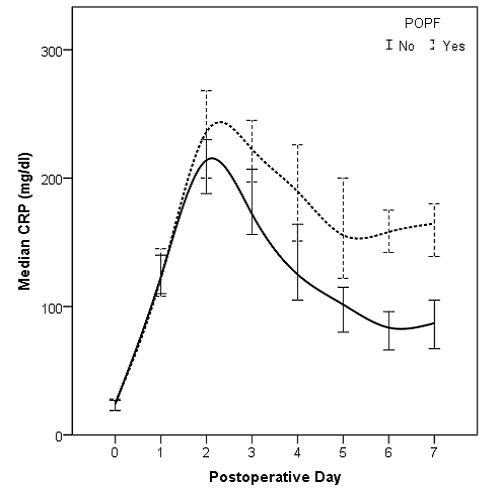
\includegraphics[width=\textwidth]{Figures/crp_comp_crp_popf_yes_no}
		\caption{POPF Absent vs. Any Grade}
		\label{fig:crp_comp_crp_popf_yes_no}
	\end{subfigure}
	\hfill
	\begin{subfigure}{0.48\textwidth}
		\centering
		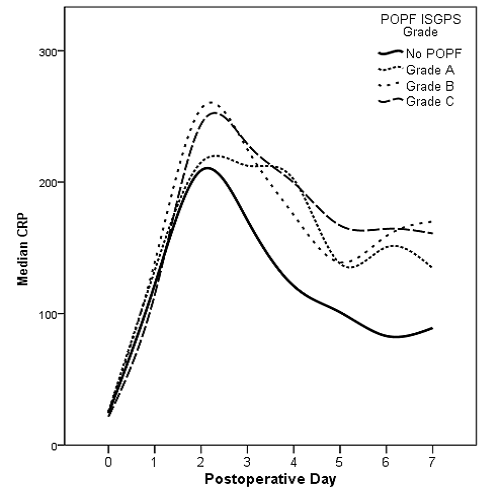
\includegraphics[width=\textwidth]{Figures/crp_comp_crp_popf_isgps}
		\caption{POPF ISGPS Grades}
		\label{fig:crp_comp_crp_popf_isgps}
	\end{subfigure}
\end{figure}
\hfill
%06/07/15 - Started this table
\begin{table}[h]
	\centering
	\caption{The relationship between CRP during the first postoperative week and post-operative pancreatic fistula (POPF) in patients undergoing pancreaticoduodenectomy.}
	\label{table:crp_comp_vs_POPF_ISGPS_p_values_only}
	\renewcommand{\arraystretch}{1.2} %Increases space between rows
	%\setlength{\tabcolsep}{9pt} %sets the space between columns
	\begin{tabular}{| c | c c c c |}
		\hline
		           &       \multicolumn{4}{c|}{POPF ISGPS Grades - \textit{p}}        \\
		Postop Day & No vs. Any Grade & No vs. A & A vs. B & B vs. C                 \\ \hline
		0          & 0.722            & 0.582    & 0.849   & 0.730                   \\
		1          & 0.242            & 0.331    & 0.740   & 0.295                   \\
		2          & 0.002            & 0.161    & 0.222   & 0.563                   \\
		3          & $<$0.001         & 0.022    & 0.602   & 0.530                   \\
		4          & $<$0.001         & 0.007    & 0.906   & 0.834                   \\
		5          & $<$0.001         & 0.035    & 0.611   & 0.959                   \\
		6          & $<$0.001         & 0.012    & 0.638   & 0.781                   \\
		7          & $<$0.001         & 0.006    & 0.235   & 0.356                   \\ \hline
		\multicolumn{5}{l}{\textit{p} - Mann-Whitney U test}                         \\
		\multicolumn{5}{l}{ISGPS - International Study Group for Pancreatic Surgery}	\\
				\multicolumn{5}{l}{POPF - Postoperative Pancreatic Fistula}
	\end{tabular}
	
	
\end{table}
%==============================================================================

%Ability of CRP to predict infectious complications in leak vs. no leak complications
%Rationale - POPF is diagnosed with a separate definition - ISGPS on Day 3. Therefore, there is no role for CRP in diagnosing POPF. Above results show that it does not discriminate between the grades either. Therefore, the following analysis is to find out if the first week CRP has any role in predicting other outcome measures.

%========================CRP vs Infections====================================
%CRP trends vs infections in patients with or without popf in a 2-panel figure and table showing median, iqr and p-values below it
\clearpage
\begin{figure}[t]
	\caption{Relationship between postoperative CRP and clinically significant infectious complications in patients without (A) and with (B) POPF.}
	\label{fig:crp_comp_infectious_leak}
	\centering
	\begin{subfigure}{0.48\textwidth}
		\centering
		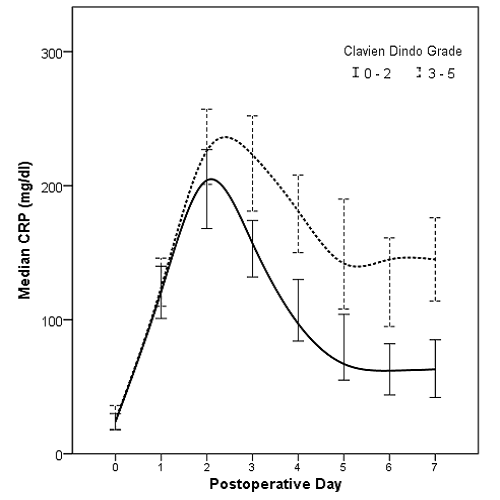
\includegraphics[width=\textwidth]{Figures/crp_comp_infectious_leak0}
		\caption{Patients with \textbf{\underline{no}} POPF}
		\label{fig:crp_comp_infectious_leak0}
	\end{subfigure}
	\hfill
	\begin{subfigure}{0.48\textwidth}
		\centering
		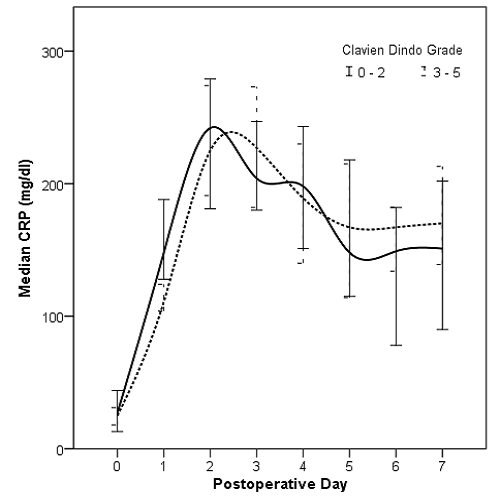
\includegraphics[width=\textwidth]{Figures/crp_comp_infectious_leak1}
		\caption{Patients with POPF}
		\label{fig:crp_comp_infectious_leak1}
	\end{subfigure}
\end{figure}
\vfill
%07/07/15 - Started this table
\begin{table}[h]
	\centering
	\caption{The relationship between postoperative CRP and infectious complications grouped by POPF. (Mann-Whitney U test)}
	\label{table:crp_comp_vs_infections_popf_y1n0}
	%\renewcommand{\arraystretch}{1.1} %Increases space between rows
	%\setlength{\tabcolsep}{9pt} %sets the space between columns
	\begin{tabular}{| c | c c c | c c c |}
		\hline
		           &       \multicolumn{3}{c}{POPF Absent}       &      \multicolumn{3}{c}{POPF Present}       \\
		           & \multicolumn{3}{c}{Infectious Complication} & \multicolumn{3}{c}{Infectious Complication} \\
		Postop Day & No          & Yes         & p               & No          & Yes         & p               \\
		           & (n=85)      & (n=41)      &                 & (n=19)      & (n=43)      &  \\ \hline
		0          & 24          & 25          & 0.379           & 27          & 25          & 0.629           \\
		           & (12 - 42)   & (14 - 41)   &                 & (13 - 44)   & (16 - 34)   &  \\
		1          & 122         & 123         & 0.667           & 148         & 116         & 0.038           \\
		           & (85 - 156)  & (87 - 148)  &                 & (114 - )    & (94 - 161)  &  \\
		2          & 204         & 218         & 0.203           & 242         & 228         & 0.919           \\
		           & (136 - 242) & (165 - 262) &                 & (181 - 279) & (186 - 296) &  \\
		3          & 157         & 213         & 0.011           & 206         & 226         & 0.846           \\
		           & (105 - 211) & (150 - 258) &                 & (180 - 297) & (175 - 281) &  \\
		4          & 97          & 173         & $<$0.001        & 214         & 190         & 0.559           \\
		           & (71 - 174)  & (118 - 216) &                 & (151 - 250) & (137 - 252) &  \\
		5          & 76          & 122         & $<$0.001        & 140         & 167         & 0.639           \\
		           & (40 - 129)  & (87 - 202)  &                 & (115 - 218) & (111 - 222) &  \\
		6          & 64          & 121         & $<$0.001        & 148         & 168         & 0.275           \\
		           & (31 - 133)  & (87 - 172)  &                 & (78 - 182)  & (109 - 224) &  \\
		7          & 62          & 141         & $<$0.001        & 158         & 167         & 0.644           \\
		           & (25 - 106)  & (90 - 190)  &                 & (90 - 231)  & (101 - 226) &  \\ \hline
		\multicolumn{7}{l}{Values are median (inter-quartile range.)}                                          \\
		\multicolumn{7}{l}{p - Mann-Whitney U test)}
	\end{tabular}
\end{table}
%==============================================================================

%========================ROC Curves==========================================
\clearpage
\begin{figure}[t]
	\caption{Receiver operating characteristics curve analysis of C-reactive protein as a marker of postoperative infective complications.}
	\label{fig:crp_comp_ROC_infection}

	\centering
	\begin{subfigure}{0.3\textwidth}
		\centering
		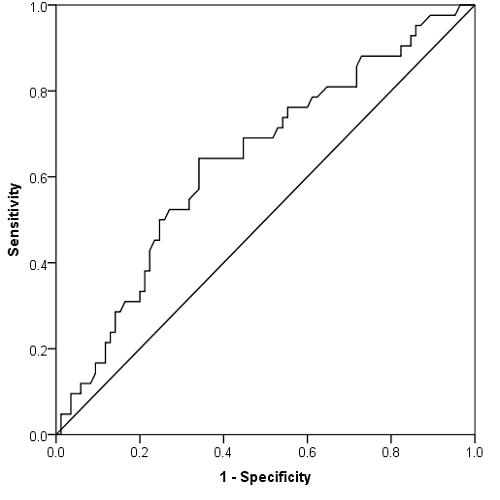
\includegraphics[width=\textwidth]{Figures/crp_comp_ROC_infection_D3}
		\caption{Day 3}
		\label{fig:crp_comp_ROC_infection_D3}
	\end{subfigure}
	\hfill
	\begin{subfigure}{0.3\textwidth}
		\centering
		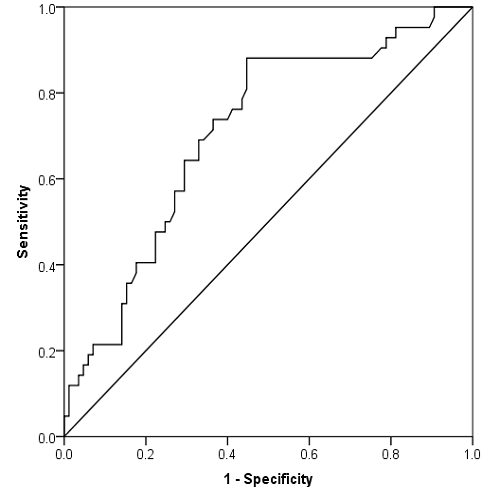
\includegraphics[width=\textwidth]{Figures/crp_comp_ROC_infection_D4}
		\caption{Day 4}
		\label{fig:crp_comp_ROC_infection_D4}
	\end{subfigure}
	\hfill
	\begin{subfigure}{0.3\textwidth}
		\centering
		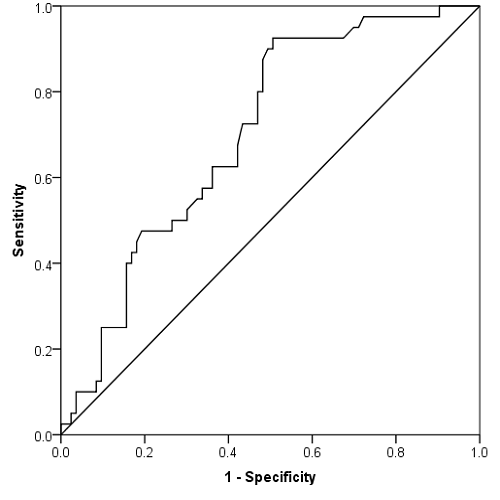
\includegraphics[width=\textwidth]{Figures/crp_comp_ROC_infection_D5}
		\caption{Day 5}
		\label{fig:crp_comp_ROC_infection_D5}
	\end{subfigure}
	\begin{subfigure}{0.3\textwidth}
		\centering
		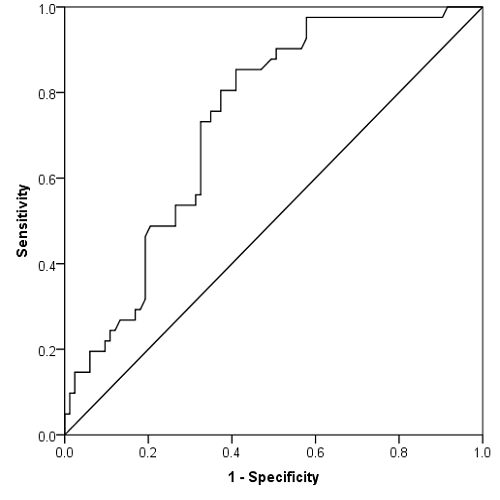
\includegraphics[width=\textwidth]{Figures/crp_comp_ROC_infection_D6}
		\caption{Day 6}		
		\label{fig:crp_comp_ROC_infection_D6}
	\end{subfigure}
	\begin{subfigure}{0.3\textwidth}
		\centering
		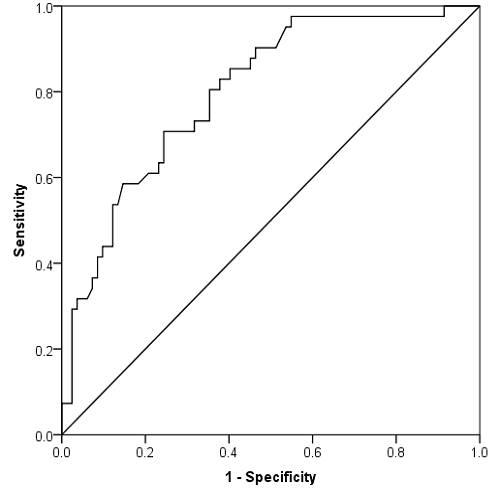
\includegraphics[width=\textwidth]{Figures/crp_comp_ROC_infection_D7}
		\caption{Day 7}
		\label{fig:crp_comp_ROC_infection_D7}
	\end{subfigure}
\end{figure}
\vfill
%07/07/15 - Started this table
\begin{table}[h]
	\centering
	\caption{Receiver operating characteristics curve analysis of C-reactive protein as a marker of postoperative infective complications in patients who did not develop a POPF}
	\label{table:crp_comp_ROC_infections_noPOPF}
	\renewcommand{\arraystretch}{1.4} %Increases space between rows
	%\setlength{\tabcolsep}{9pt} %sets the space between columns
	\begin{tabular}{| c | c c c | c c c c c |}
		\hline
		Day & AUC  & p        & 95\% CI     & CRP & Spec. & Sens. & NPV  & PPV               \\ \hline
		3   & 0.64 & 0.011    & 0.54 - 0.74 & 178 & 0.66  & 0.64  & 0.79 & 0.48              \\
		4   & 0.71 & $<$0.001 & 0.61 - 0.80 & 125 & 0.64  & 0.74  & 0.83 & 0.50              \\
		5   & 0.70 & $<$0.001 & 0.61 - 0.80 & 107 & 0.64  & 0.63  & 0.78 & 0.45              \\
		6   & 0.73 & $<$0.001 & 0.65 - 0.82 & 92  & 0.68  & 0.73  & 0.84 & 0.53              \\
		7   & 0.80 & $<$0.001 & 0.72 - 0.88 & 87  & 0.65  & 0.81  & 0.87 & 0.52              \\ \hline
		\multicolumn{9}{l}{AUC - Area under curve, Spec. - Specificity, Sens. - Sensitivity} \\
		\multicolumn{9}{l}{NPV - Negative Predictive Value, PPV - Positive Predictive Value}
	\end{tabular}
\end{table}

%=============================================================================
%Quick analysis of CPET vs postop CRP - maybe one table
%ROC analysis of CRP vs LOS
%Multivariate analysis of CRP as continuous or categorical vs complications, 
\clearpage
\section{Discussion}